\documentclass{beamer}

%% slide-specific

\usetheme[progressbar=frametitle]{metropolis}
%\usecolortheme{spruce}
%\metroset{block=fill}

% define Metropolis colors    
\definecolor{mAlert}{HTML}{EB811B}
\definecolor{mExample}{HTML}{14B03D}
\definecolor{mBlock}{HTML}{23373b}

% my blocks
\setlength\fboxsep{0pt}%

\newcommand{\myblock}[1]{\colorbox{mBlock!8}{\begin{minipage}{\linewidth}#1\end{minipage}}}
\newcommand{\myblockmath}[1]{\colorbox{mBlock!8}{\begin{minipage}{\linewidth}\vspace{-6pt}#1\end{minipage}}}
\newcommand{\myblockinline}[1]{\colorbox{mBlock!8}{#1}}
\newcommand{\myexample}[1]{\colorbox{mExample!8}{\begin{minipage}{\linewidth}#1\end{minipage}}}
\newcommand{\myexamplemath}[1]{\colorbox{mExample!8}{\begin{minipage}{\linewidth}\vspace{-6pt}#1\end{minipage}}}
\newcommand{\myexampleinline}[1]{\colorbox{mExample!8}{#1}}
\newcommand{\myalert}[1]{\colorbox{mAlert!8}{\begin{minipage}{\linewidth}#1\end{minipage}}}
\newcommand{\myalertmath}[1]{\colorbox{mAlert!8}{\begin{minipage}{\linewidth}\vspace{-6pt}#1\end{minipage}}}
\newcommand{\myalertinline}[1]{\colorbox{mAlert!8}{#1}}

%% other
\newcommand{\mystructure}[1]{\mathcal{#1}}




%% packages
\usepackage{amsmath,amssymb,amsthm}
\usepackage{booktabs}
\usepackage[czech]{babel}
\usepackage{enumerate}
\usepackage{forest}
\usepackage{multicol}
% \usepackage{tcolorbox}
\usepackage{tikz}
    \usetikzlibrary{arrows.meta}
%\usepackage[unicode]{hyperref}
\usepackage[utf8x]{inputenc}
\usepackage{xfrac}

% %% theorems
% \theoremstyle{plain}
%     \newtheorem{theorem}{Věta}[section]
%     \newtheorem*{theorem-unnumbered}{Věta}
%     \newtheorem{proposition}[theorem]{Tvrzení}
%     \newtheorem{corollary}[theorem]{Důsledek}
%     \newtheorem{lemma}[theorem]{Lemma}
%     \newtheorem{observation}[theorem]{Pozorování}
% \theoremstyle{definition}
%     \newtheorem{definition}[theorem]{Definice}
%     \newtheorem*{algorithm}{Algoritmus}
% \theoremstyle{remark}
%     \newtheorem{remark}[theorem]{Poznámka}
%     \newtheorem{example}[theorem]{Příklad}
%     \newtheorem{exercise}{Cvičení}[chapter]
%     \newtheorem*{solution}{Řešení}

%% macros and definitions
\DeclareMathOperator{\Aut}{Aut}
\DeclareMathOperator{\Conseq}{Csq}
\DeclareMathOperator{\DeLO}{DeLO}
\DeclareMathOperator{\dom}{dom}
\DeclareMathOperator{\Fm}{Fm}
\DeclareMathOperator{\M}{M}
%\DeclareMathOperator{\Proof}{Proof}
\DeclareMathOperator{\rng}{rng}
\DeclareMathOperator{\Term}{Term}
\DeclareMathOperator{\Th}{Th}
\DeclareMathOperator{\Thm}{Thm}
\DeclareMathOperator{\Tree}{Tree}
\DeclareMathOperator{\Var}{Var}
\DeclareMathOperator{\VF}{VF}

\newcommand{\A}{\structure{A}}
\newcommand{\B}{\structure{B}}
\newcommand{\Con}{\mathit{Con}}
\newcommand{\disjointunion}{\mathbin{\dot{\sqcup}}}
\newcommand{\F}{\ensuremath{\mathrm{F}}}
\newcommand{\landsymb}{{\land}}
\newcommand{\lbin}{\mathbin{\square}}
\newcommand{\lbinsymb}{{\lbin}}
\newcommand{\liff}{\mathbin{\leftrightarrow}}
\newcommand{\liffsymb}{{\liff}}
\newcommand{\limplies}{\mathbin{\rightarrow}}
\newcommand{\limpliessymb}{{\limplies}}
\newcommand{\lorsymb}{{\lor}}
\newcommand{\Prf}{\mathit{Prf}}
\newcommand{\proves}{\vdash}
%\newcommand{\structure}[1]{\mathcal{#1}}
\newcommand{\todo}{[TODO]}
\newcommand{\T}{\ensuremath{\mathrm{T}}}
\newcommand{\union}{\mathbin{\cup}}


\title{První přednáška}
\subtitle{NAIL062 Výroková a predikátová logika}
\author{Jakub Bulín (KTIML MFF UK)}
% \institute{KTIML MFF UK}
\date{Zimní semestr 2024}


\begin{document}


\maketitle


\begin{frame}{Jak se učit?}

    Velmi doporučuji tento online minikurz o efektivním učení:


    \href{https://www.samford.edu/departments/academic-success-center/how-to-study}{\alert{https://www.samford.edu/departments/academic-success-center/how-to-study}}

    Investujte 35 minut nyní, ušetřete mnoho hodin později!
    
\end{frame}


\begin{frame}{Cesta k jistému úspěchu u zkoušky}

    \begin{itemize}    
        \item \alert{Před přednáškou} alespoň zběžně projděte skripta, snažte se pochopit motivaci a smysl definic a hlavních tvrzení.
        \item Po přednášce skripta \alert{podrobně přečtěte}, nejasnosti ujasněte.
        \item Ujistěte se, že umíte pracovat i s \alert{formalizmem}.
        \item Věnujte pozornost i \alert{cvičení}, pomůže vám vše pochopit.
        \item Studujte \alert{průběžně}, a průběžně \alert{testujte své znalosti}.
    \end{itemize}

\end{frame}


\begin{frame}{První přednáška}

    \textbf{Program}
        \begin{itemize}
            \item úvod do logiky
            \item neformální představení výrokové a predikátové logiky (``upoutávka'')
            \item syntaxe výrokové logiky
            \item sémantika výrokové logiky (začátek)
        \end{itemize}

    \textbf{Materiály}

        \href{https://github.com/jbulin-mff-uk/nail062/raw/main/lecture/lecture-notes/lecture-notes.pdf}{\alert{\textbf{Zápisky z přednášky}}}, Kapitola 1 a Sekce 2.1-2.2.4 z Kapitoly 2

\end{frame}


\section{\sc Kapitola 1: Úvod do logiky}


\begin{frame}{Co je logika?}

    % 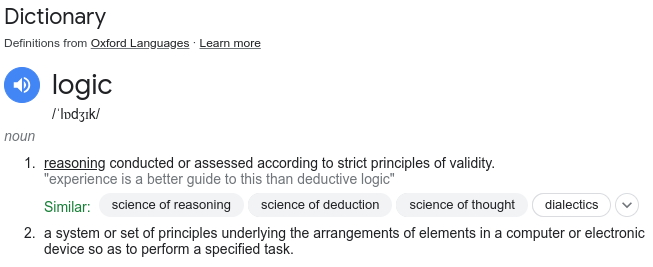
\includegraphics[width=\textwidth]{slides1-images/definiton-of-logic.png}
    
    \href{https://www.google.com/search?q=define+logic}{\textbf{Dvě definice:}}
        \begin{enumerate}
            \item soubor principů, které jsou základem uspořádání prvků nějakého systému (např. programu, zařízení, protokolu)
            \item věda o uvažování prováděném podle striktních pravidel zachovávajících platnost 
        \end{enumerate}
        
    \medskip 
    
    \pause

    \myblock{\textbf{V informatice obojí:} daný systém nejprve \emph{formálně popíšeme}, a poté o něm \emph{formálně uvažujeme} (automaticky!), tj. odvozujeme \alert{platné inference} za použití nějakého \alert{dokazovacího systému}
    }

\end{frame}


\begin{frame}{Historie a aplikace logiky}

    {\footnotesize Filozofie $\to$}  {\normalsize Matematika $\to$}  {\Large Teoretická informatika $\to$} 
    
    \medskip
    
    \myalertinline{\Huge Aplikovaná informatika}

    \pause

    \medskip

    \begin{itemize}
        \item logic programming
        \item discrete optimization (SAT solving, scheduling, planning)
        \item database theory
        \item verification (software, hardware, protocol)
        \item automated reasoning and proving
        \item knowledge-based representation
        \item artificial intelligence
    \end{itemize}

\end{frame}


\section{1.1 Výroková logika}


\begin{frame}{Příklad ze života: Hledání pokladu}

    \myexample{
        Při hledání pokladu jsme narazili na rozcestí dvou chodeb. Víme, že na konci každé chodby je buď poklad, nebo drak, ale ne obojí. 
        
        \pause

        \medskip
        Trpaslík nám řekl, že: 
        \begin{itemize}
            \item \emph{``Alespoň jedna z těch dvou chodeb vede k pokladu''}, a že
            \item \emph{``První chodba vede k drakovi.''}
        \end{itemize}

        \pause

        \medskip
        Je známo, že trpaslíci buď vždy mluví pravdu, nebo vždy lžou. Kterou cestou se máme vydat?
    }

\end{frame}


\begin{frame}{Výroky neformálně}

    \alert{Výrok} je tvrzení, kterému lze přiřadit pravdivostní hodnotu: 
    \begin{center}
        \alert{pravdivý} (\emph{True}, 1), nebo \alert{lživý} (\emph{False}, 0)
    \end{center}

    \pause
    
    \alert{Prvovýroky} (\alert{atomické výroky}, \alert{výrokové proměnné}) zkombinované pomocí logických spojek a závorek do \alert{složených výroků}:

    \pause

    \myexample{
        ``(Trpaslík lže,) \emph{právě když} (druhá chodba vede k drakovi.)''\
    }
    
    \medskip

    \pause

    \begin{description}\setlength{\itemsep}{3pt}
        \item[\LARGE\alert{$\neg$}] ``neplatí X'', \emph{negace}
        \item[\LARGE\alert{$\landsymb$}] ``X a Y'', \emph{konjunkce}
        \item[\LARGE\alert{$\lorsymb$}] ``X nebo Y'', \emph{disjunkce} (není exkluzivní)
        \item[\LARGE\alert{$\limpliessymb$}] ``pokud X, potom Y'', \emph{implikace} (čistě logická)
        \item[\LARGE\alert{$\liffsymb$}] ``X, právě když Y'', \emph{ekvivalence}
    \end{description}

\end{frame}


\begin{frame}{Formalizace ve výrokové logice}

    Volba množiny prvovýroků: \myalertinline{bity informace popisující daný systém}

    \pause
    
    \myexample{            
        $p_1=${\it ``Poklad je v první chodbě.''}\\
        $p_2=${\it ``Poklad je ve druhé chodbě.''}
    }

    \pause

    (Co nejmenší, např. hodnota $t=${\it ``Trpaslík mluví pravdu.''} je jednoznačně určená hodnotami $\mathbb P=\{p_1,p_2\}$.)
    
    \pause

    \begin{itemize}
        \item {\it Poklad nebo drak, ale ne obojí}: zakódované do volby $\mathbb P$ (přítomnost draka je absence pokladu)
        \item {\it ``První chodba vede k drakovi.''} $\Leftrightarrow$ \alert{$\neg p_1$}
        \item {\it ``Alespoň jedna z chodeb vede k pokladu.''} $\Leftrightarrow$ \alert{$p_1 \lor p_2$}
        \item {\it Trpaslík buď mluví pravdu, nebo lže}:
        \myexamplemath{
        $$
        \varphi = (\neg p_1 \land (p_1 \lor p_2)) \lor (\neg (\neg p_1) \land \neg (p_1 \lor p_2))
        $$
        }
    \end{itemize}

    \pause

    \medskip
    \myblock{
    \alert{Teorie} $T=\{ \varphi \}$ v \alert{jazyce} $\mathbb P=\{p_1,p_2\}$, $\varphi$ je \alert{axiom} $T$.
    }

\end{frame}


\begin{frame}{Modely a důsledky}

    Lze určit, kde je poklad? Je $p_1$ nebo $p_2$ \alert{důsledkem} $\varphi$ resp. $T$?    

    \alert{``Svět''}, ve kterém je např. v první chodbě poklad a ve druhé drak, popíšeme pomocí \alert{pravdivostního ohodnocení} $p_1=1,p_2=0$, neboli \alert{modelu} $v=(1,0)$ jazyka $\mathbb P$. Celkem máme 4 ``světy'' a modely:
    \myexample{\vspace{-6pt}
    $$
    \M_\mathbb P=\{(0,0),(0,1),(1,0),(1,1)\}.
    $$
    }

    \pause

    Je ``svět'' popsaný modelem $v = (1,0)$ \emph{konzistentní} s tím, co víme, tj. \alert{platí} v modelu $v$ výrok $\varphi$ resp. teorie $T$? Vyhodnotíme podle stromové struktury $\varphi$:
    $$
    v(p_1) = 1,\ v(p_2) = 0,\ v(\neg p_1) = 0,\ v(p_1 \lor p_2)=1,\ \dots,\ \alert{v(\varphi)=0}
    $$
    
    \pause

    Množina \alert{modelů výroku} \( \varphi \) (resp.\ \emph{modelů teorie} \( T \)):
    \myexample{\vspace{-6pt}
    $$
    \M_\mathbb P(\varphi)=\M_\mathbb P(T)=\{(0,1)\}.
    $$
    }

    \myblock{V \alert{každém modelu} teorie $T$ platí výrok $p_2$, neboli $p_2$ je \alert{důsledek}~$T$.}
    
\end{frame}


\begin{frame}{Dokazovací systémy}

    Ověřovat všechny modely je nepraktické, pro $|\mathbb P|=n$ máme $2^n$ modelů, a $\mathbb P$ může být i nekonečná.

    \pause

    \textbf{Dokazovací systém}
    \begin{itemize}
        \item \alert{důkaz} výroku~\( \psi \) z teorie \(T\) je formálně definovaný syntaktický objekt, snadno (mechanicky) ověřitelný
        \item lze hledat algoritmicky čistě na základě struktury \( \psi \) a axiomů \(T\) (``\emph{syntaxe}''), nemusíme se zabývat modely (``\emph{sémantikou}'').
    \end{itemize}        
    
    \pause
    Klíčové vlastnosti:

    \pause
    \myblock{
    \begin{itemize}
        \item \alert{korektnost}: pokud existuje důkaz \( \psi \) z \(T\), potom \( \psi \) platí v \(T\)
        \item \alert{úplnost}, pokud \( \psi \) platí v \(T\), potom existuje důkaz \( \psi \) z \(T\)
    \end{itemize}
    }

    \pause
    %Korektnost je nutná, ale efektivní dokazovací systém může být užitečný, i pokud v něm nelze dokázat vše, co platí.
    Ukážeme si \alert{metodu analytického tabla} a \alert{rezoluční metodu}. Obě dokazují \emph{sporem}: předpokládají platnost $T$ a \( \neg \psi \), hledají spor.

\end{frame}


\begin{frame}{Metoda analytického tabla}

\begin{itemize}
    \item důkaz je strom olabelovaný předpoklady o platnosti výroků
    \item v kořeni: \alert{neplatí} dokazovaný výrok $\psi$ (důkaz sporem)
    \item připojíme platnost axiomů z $T$
    
    \pause
    \item při konstrukci zjednodušujeme výroky ve vrcholech, \alert{invariant}:
    
    \pause
    \bigskip
    \myalert{\it
        Každý model teorie \(T\), ve kterém neplatí \(\psi\), se musí \emph{shodovat} s některou z větví tabla. 
    }

    \pause
    
    \bigskip

    např.:
    
    \bigskip
    \myblock{
    \alert{\small True $(\varphi_1 \limplies \varphi_2 )$} zredukujeme rozvětvením na \alert{\small False $\varphi_1$} a \alert{\small True $\varphi_2$},\\
    \alert{\small False $(\varphi_1 \limplies \varphi_2 )$} zredukujeme připojením \alert{\small True $\varphi_1$} a \alert{\small False $\varphi_2$}.
    }
    \smallskip    
        
    \pause

    \item \alert{sporná} větev = předpokládá True i False stejného výroku
    \item \alert{důkaz} = všechny větve sporné (tj. nemůže existovat model $T$, ve kterém neplatí $\psi$)
\end{itemize}

\end{frame}


\begin{frame}{Příklad tablo důkazu}

    \vspace{-6pt}
    \begin{figure}\scalebox{0.8}{\small
        \centering
        \begin{forest}
        [False \( p_2 \)
            [True \( (\neg p_1 \land (p_1 \lor p_2)) \lor (\neg (\neg p_1) \land \neg (p_1 \lor p_2)) \) 
                [True \( \neg p_1 \land (p_1 \lor p_2) \)
                    [True \( \neg p_1 \)
                        [True \( p_1 \lor p_2 \)
                            [False \( p_1 \)
                                [True \( p_1 \), tikz={\node[fit to=tree,label=below:\alert{fail}] {};}
                                ]
                                [True \( p_2 \), tikz={\node[fit to=tree,label=below:\alert{fail}] {};}
                                ]
                            ]
                        ]
                    ]
                ]
                [True \( \neg (\neg p_1) \land \neg (p_1 \lor p_2) \)
                    [True \( \neg (\neg p_1) \)
                        [True \(\neg (p_1 \lor p_2) \)
                            [False \( (\neg p_1) \)
                                [True \( p_1 \)
                                    [False \(p_1 \lor p_2 \)
                                        [False \(p_1\)
                                            [False \(p_2\), tikz={\node[fit to=tree,label=below:\alert{fail}] {};}
                                            ]
                                        ]
                                    ]
                                ]
                            ]
                        ]
                    ]
                ]
            ]
        ]
        \end{forest}

    }
    \end{figure}    

\end{frame}


\begin{frame}{Konjunktivní normální forma (CNF)}

    \alert{literál} $p$, $\neg p$\hfill \alert{klauzule} disjunkce literálů\hfill \alert{CNF} konjunkce klauzulí

    \myblock{
        každý výrok má \alert{ekvivalentní} CNF (\alert{$\psi \sim \psi'$}, stejné modely)
    }
    
    \pause
    \myexample{např. pro výrok 
    $
    (\neg p_1 \land (p_1 \lor p_2)) \lor (\neg (\neg p_1) \land \neg (p_1 \lor p_2))
    $
    }

    \pause
    nahradíme \alert{$\neg (\neg p_1) \sim p_1$} a \alert{$\neg (p_1 \lor p_2) \sim (\neg p_1 \land \neg p_2)$} (\emph{De Morgan})

    \pause
    \myexamplemath{
    $$
    (\neg p_1 \land (p_1 \lor p_2)) \lor (p_1 \land \neg p_1 \land \neg p_2)
    $$
    }

    \pause
    a dále opakovaně použijeme \alert{distributivitu} \( \lorsymb \) vůči \( \landsymb \): \medskip

    \pause
    \myexampleamsmath{
    \begin{gather*}
    (\neg p_1 \lor p_1) \land (\neg p_1 \lor \neg p_1) \land (\neg p_1 \lor \neg p_2) \land (p_1 \lor p_2 \lor p_1) \land\\ (p_1 \lor p_2 \lor \neg p_1)\land (p_1 \lor p_2 \lor \neg p_2)    
    \end{gather*}    
    }

    \pause
    už je CNF, ještě zjednodušíme: odstraníme duplicitní literály, a klauzule obsahující $p_i$ a zároveň $\neg p_i$ (to jsou \alert{tautologie})

    \pause
    \myexamplemath{
    $$
    \neg p_1 \land (\neg p_1 \lor \neg p_2) \land (p_1 \lor p_2)
    $$
    }

\end{frame}


\begin{frame}{Rezoluční důkaz}

    Dk sporem, převeď \alert{negaci} dokazovaného do CNF a přidej k $T$

    \pause
    \myblock{
    \alert{\(p_2\) platí v \(T\)}, právě když je následující CNF výrok \alert{nesplnitelný}:
    }

    \myexamplemath{
    $$
    \neg p_1 \land (\neg p_1 \lor \neg p_2) \land (p_1 \lor p_2)\land\alert{\neg p_2}
    $$
    }

    \pause
    množinový zápis:
    \myexampleinline{$
    S=\left \{ \{\neg p_1\},\{\neg p_1,\neg p_2\},\{p_1, p_2\},\{\neg p_2\} \right \}
    $
    }

    \pause
    \medskip

    \myalert{\alert{rezoluční pravidlo}: je-li $p\in C_1$ a $\neg p\in C_2$, potom \emph{rezolventa} 
    $$
    C= (C_1\setminus \{p\})\cup(C_2\setminus \{\neg p\})
    $$ platí v každém modelu, ve kterém platí $C_1$ i $C_2$
    }
    
    \pause
    \medskip

    \alert{rezoluční zamítnutí $S$}: posloupnost klauzulí, kde každá je buď z $S$ nebo rezolventa předchozích, poslední je prázdná klauzule $\square$

    \pause
    \myblock{\textbf{myšlenka:} protože $\square$ nemá žádný model, je i $S$ nesplnitelná}

\end{frame}


\begin{frame}{Příklad rezolučního důkazu}

    \alert{rezoluční zamítnutí} (3. klauzule je rezolventou 1.\&2., 5. je z 3.\&4.)

    \myexamplemath{
    \[
        \{\neg p_1\},\{p_1, p_2\},\{p_2\},\{\neg p_2\},\square
    \]
    }

    \pause
    \bigskip

    \alert{rezoluční strom} (listy klauzule z $S$, vnitřní vrcholy rezolventy synů) 

    \myexample{
        \begin{center}
            \begin{forest}
            for tree={grow=north}
            [\( \square \)
                [\( \{\neg p_2\} \)]
                [\( \{p_2\} \)
                [{\( \{p_1, p_2\} \)}]
                [\( \{\neg p_1\} \)]
                ]
            ]
            \end{forest}
        \end{center}
    }

\end{frame}


\begin{frame}{Příklad: Barvení grafů}

    \myexample{
    Najděte vrcholové obarvení následujícího grafu třemi barvami.
    \begin{center}
    \begin{tikzpicture}[every node/.style={circle,fill=blue!10,draw,minimum size=0.5cm,node distance=1.5cm}]
    \node (1) {$1$};
    \node[right of=1] (2) {$2$};
    \node[below of=2] (3) {$3$};
    \node[left of=3] (4) {$4$};
    \path[draw] (1) -- (2) -- (3) -- (4) -- (1) -- (3);
    \end{tikzpicture}
    \end{center}
    }
    
    \pause
    graf: množina vrcholů a množina (libovolně) \alert{orientovaných} hran
    \[
    \mystructure G = \langle V; E \rangle = \langle \{1,2,3,4\}; \{(1,2),(1,3),(1,4),(2,3),(3,4)\} \rangle
    \]
    \pause
    jak formalizovat? pro $v\in V$ a $c\in C=\{R,G,B\}$:
    
    \myalertmath{
    $$
    p_v^c=\text{\it``vrchol \(v\) má barvu \(c\)''}
    $$
    }

    \pause
    \mbox{\small $\mathbb P=\{p_v^c\mid c\in C,v\in V\}=\{p_1^R,p_1^G,p_1^B,p_2^R,p_2^G,p_2^B,p_3^R,p_3^G,p_3^B,p_4^R,p_4^G,p_4^B\}$}

    \pause
    máme celkem \( |\M_\mathbb P|=2^{12}=4096 \) \alert{modelů jazyka} (12-dim. vektorů)
\end{frame}


\begin{frame}{Formalizace hranového obarvení}

    \begin{itemize}
        \item každý vrchol má nejvýše jednu barvu: $4^4=2^8=256$ modelů\medskip

        \myexamplemath{\vspace{-9pt}$$
        T_1 = \{ (\neg p_v^R \lor \neg p_v^G) \land (\neg p_v^R \lor \neg p_v^B) \land (\neg p_v^G \lor \neg p_v^B) \mid v \in V \}
        $$}

        \pause
        \medskip

        \item a každý vrchol má alespoň jednu barvu: $3^4=81$ modelů\medskip
        
        \myexamplemath{\vspace{-9pt}$$T_2 = T_1\cup \{ p_v^R \lor p_v^G \lor p_v^B \mid v \in V \}= T_1\cup \{\bigvee_{c\in C} p_v^c \mid v \in V \}
        $$}

        \pause
        \medskip
        
        \myblock{$T_2$ je \alert{extenze} teorie $T_1$ neboť \alert{každý důsledek $T_1$ platí i v $T_2$}, zde dokonce $\M_\mathbb P(T_2)\subseteq\M_\mathbb P(T_1)$}
        %\footnote{Proč $\subseteq$? Čím více vlastností požadujeme, tím méně objektů je splňuje.}

        \pause
        \medskip

        \item nakonec přidáme \alert{hranovou podmínku}:\medskip
        
        \myexamplemath{$$
        T_3 = T_2\cup \{ \bigwedge_{c\in C} 
        (\neg p_u^c \lor \neg p_v^c) \mid (u,v) \in E \}
        $$}  

        \pause
        \medskip

        Výsledná teorie \( T_3 \) je \alert{splnitelná} (má model), právě když je graf \( \mystructure{G} \) 3-obarvitelný.   
    \end{itemize}

\end{frame}


\begin{frame}{Co s ní?}

\textbf{Všechna obarvení?} 

$T_3$ má 6 modelů: \( v = (1,0,0,0,1,0,0,0,1,0,1,0) \) a další získané permutací barev \vspace{-12pt}
\begin{center}
    \begin{tikzpicture}[every node/.style={circle,fill=blue!10,draw,minimum size=0.3cm,node distance=1cm}]
    \node[fill=red] (1) {$1$};
    \node[fill=green,right of=1] (2) {$2$};
    \node[fill=blue,below of=2] (3) {$3$};
    \node[fill=green,left of=3] (4) {$4$};
    \path[draw] (1) -- (2) -- (3) -- (4) -- (1) -- (3);
    \end{tikzpicture}
\end{center}

\pause

\textbf{Obarvení, ve kterých je vrchol 1 modrý a vrchol 2 zelený?} 

Odpovídají modelům teorie \( T_3 \cup \{ p_1^B, p_2^G\} \)

\pause

\textbf{Důkaz, že vrcholy 2 a 4 musí mít stejnou barvu?}

\alert{Tablo} s kořenem $\text{False  }(p_2^R \land p_4^R)\lor(p_2^G \land p_4^G)\lor(p_2^B \land p_4^B)$

\pause

Nebo \alert{rezolucí}: přidáme \alert{negaci} \( (p_2^R \land p_4^R)\lor(p_2^G \land p_4^G)\lor(p_2^B \land p_4^B) \), vše převedeme do CNF a zamítneme

\end{frame}


\section{1.2 Predikátová logika}


\begin{frame}{Nevýhody formalizace ve výrokové logice}
Teorie $T_3$ je poměrně velká, a `natvrdo' kóduje graf $\mystructure G$.

\pause

\begin{center}
    \begin{tikzpicture}[every node/.style={circle,fill=blue!10,draw,minimum size=0.5cm,node distance=1.5cm}]
    \node (1) {$1$};
    \node[right of=1] (2) {$2$};
    \node[below of=2] (3) {$3$};
    \node[left of=3] (4) {$4$};
    \path[draw] (1) -- (2) -- (3) -- (4) -- (1) -- (3);
    \node[right of=3] (5) {$5$};
    \path[draw] (2) -- (5) -- (3);
    \end{tikzpicture}
\end{center}

\pause
Obohatit jazyk $\mathbb P'=\mathbb P \cup \{ p_5^R,p_5^G,p_5^B\}
$ a vytvořit ještě větší teorii~$T'_3$ přidáním axiomů o vrcholu 5 a hranách $(2, 5), (3,5)$?

\pause
A co vlastnosti obecně platné o všech nebo mnoha grafech?

\pause
\myblock{
V \alert{predikátové logice} můžeme mluvit \alert{o vrcholech} grafu pomocí \alert{proměnných} a přirozeně vyjádřit vlastnosti jako:
\begin{itemize}
    \item \emph{``z vrcholu \(u\) vede hrana do vrcholu \(v\)''}
    \item \emph{``vrchol \(u\) je zelený''}
\end{itemize}
}
\end{frame}


\begin{frame}{Predikátová logika: struktury a jazyk}

    \textbf{Modely} už nejsou 0--1 vektory, ale \alert{struktury}, např. naše (orientované) grafy:

    \myexampleamsmath{\footnotesize\vspace{6pt}\begin{align*}
        &\mystructure G = \langle V^\mystructure G; E^\mystructure G \rangle = \langle \{1,2,3,4\}; \{(1,2),(1,3),(1,4),(2,3),(3,4)\} \rangle \\ 
        &\mystructure{G}' = \langle V^{\mystructure{G}'}; E^{\mystructure{G}'} \rangle = \langle \{1,2,3,4,5\}; \{(1,2),(1,3),(1,4),(2,3),(3,4),(2,5),(3,5)\} \rangle
    \end{align*}
    }

    \pause
    \begin{itemize}
        \item množina vrcholů, a binární relace na této množině
        \pause
        \item \alert{jazyk} specifikuje kolik \alert{relací} jakých arit má struktura mít, a symboly pro ně
        \pause
        \item např. \alert{jazyk grafů} \( \mathcal L=\langle E \rangle \) (kde \(E\) je binární relační symbol)
        \pause
        \item $\mystructure G$ a $\mystructure G'$ jsou \alert{struktury v jazyce} $\mathcal L$ (\alert{$\mathcal L$-struktury})   
        \pause
        \item můžeme mít také \alert{funkce} a \alert{konstanty}, a symbol \alert{$=$} pro \alert{rovnost} 
    \end{itemize}

\end{frame}


\begin{frame}{Predikátová logika: syntaxe a sémantika}

    \textbf{Syntaxe}: místo prvovýroků \alert{atomické formule}, např. $E(x,y)$, kde $x,y$ jsou \alert{proměnné} reprezentující vrcholy; stejné logické spojky, ale navíc \alert{kvantifikátory}:
  
    \pause
    \myalert{
    \begin{description}
        \item[\alert{\( (\forall x) \)}] {\it``pro všechny vrcholy \(x\)''}
        \item[\alert{\( (\exists y) \)}] {\it``existuje vrchol \(y\)''}
    \end{description}
    }

    \pause
    (hrají roli ``konjunkce'' a ``disjunkce'' přes všechny prvky)
    
    \pause
    \bigskip

    \myexample{
    \begin{itemize}
        \item ``V grafu nejsou smyčky'': \alert{$(\forall x)(\neg E(x,x))$}
        \item ``Existuje vrchol výstupního stupně 1'': 
        \alert{$(\exists x)(\exists y)(E(x,y) \land (\forall z)(E(x,z) \limplies y=z))$}
    \end{itemize}    
    }

    \pause
    \bigskip

    \textbf{Sémantika}: V daném grafu \(\mystructure{G}\) a při \alert{dosazení} vrcholu \(u\) za proměnnou \(x\) a vrcholu \(v\) za proměnnou \(y\) \alert{vyhodnotíme} \( E(x,y) \) jako \alert{True}, právě když \alert{\( (u,v)\in E^{\mystructure{G}} \)}.
        
\end{frame}


\begin{frame}{Barvení grafů v predikátové logice}
      
    Jazyk \alert{\( \mathcal L' =\langle E, R, G, B \rangle \)}, kde \(E\) je binární a \(R,G,B\) jsou unární relační symboly (\(R(x)\) znamená {\it``vrchol \(x\) je červený''}) 

    \pause

    \alert{$\mathcal L'$-struktura}: graf s trojicí množin vrcholů

    \pause

    \vspace{-32pt}
    \begin{flushright}
        \scalebox{0.75}{
            \tikz[every node/.style={circle,fill=blue!10,draw,minimum size=0.3cm,node distance=1cm}]{
            \node[fill=red] (1) {$1$};
            \node[fill=green,right of=1] (2) {$2$};
            \node[fill=blue,below of=2] (3) {$3$};
            \node[fill=green,left of=3] (4) {$4$};
            \path[draw] (1) -- (2) -- (3) -- (4) -- (1) -- (3);
            }
        }
    \end{flushright}

    \pause

    \myexampleamsmath{\vspace{3pt}\small
    \begin{align*}
    \mystructure G_C &= \langle V^{\mystructure G_C}; E^{\mystructure G_C}, R^{\mystructure G_C}, G^{\mystructure G_C}, B^{\mystructure G_C} \rangle \\
    &= \langle \{1,2,3,4\}; \{(1,2),(1,3),(1,4),(2,3),(3,4)\}, \alert{\{1\}, \{2,4\}, \{3\}} \rangle    
    \end{align*}
    }  

    \pause
    \( \mystructure{G}_C \) je \alert{expanze} \(\mathcal L\)-struktury \( \mystructure{G} \) \alert{do jazyka} \( \mathcal L' \)

    \bigskip

    \pause
    Nejvýše jedna barva, alespoň jedna barva, hranová podmínka:

    \pause
    \myexample{\small
    \begin{itemize}
        \item $(\forall x)((\neg R(x) \lor \neg G(x)) \land (\neg R(x) \lor \neg B(x)) \land (\neg G(x) \lor \neg B(x)))$
        \item $(\forall x)(R(x) \lor G(x) \lor B(x))$
        \item $(\forall x)(\forall y)(E(x,y) \limplies ((\neg R(x) \lor \neg R(y)) \land (\neg G(x) \lor \neg G(y)) \land (\neg B(x) \lor \neg B(y))))$
    \end{itemize}
    }

\end{frame}


\section{1.3 Další druhy logických systémů}


\begin{frame}{Predikátové logiky vyšších řádů}

    \begin{itemize}[<+->]
        \item Predikátová logika, kde proměnné reprezentují jednotlivé vrcholy, je logika \alert{prvního řádu} (\alert{first-order}, \alert{FO})
        \item Logika \alert{druhého řádu} (\alert{second-order}, \alert{SO}): proměnné i pro množiny vrcholů a $n$-tic vrcholů (tj. relace, funkce)
        \bigskip

        % \myexample{\it
        %     ``Každá neprázdná zdola omezená podmnožina má infimum.''
        %     {\small
        %     \begin{align*}
        %     &(\forall S)((\exists x)S(x) \land (\exists x)(\forall y)(S(y) \limplies x\leq y) \limplies  {}\\ 
        %     &(\exists x)((\forall y)(S(y) \limplies x\leq y) \land (\forall z)((\forall y)(S(y) \limplies z\leq y)\limplies z\leq x)))
        %     \end{align*}
        %     }
        % }
        \pause
        \myexamplemath{
        $$(\exists S)(\forall x)(\forall y)(E(x,y)\limplies (S(x)\liff\neg S(y)))$$
        }  
        \pause    
        \begin{center}
            \it ``Graf je bipartitní.''
        \end{center}  

        \pause
        \medskip
        \item A v logice \emph{třetího řádu} máme i množiny množin (např. v topologii).
    \end{itemize}

\end{frame}


\begin{frame}{Logiky zobecňující pojem pravdy}
    Kromě toho lze zobecnit pojem platnosti (pravdy):
    
    \begin{itemize}[<+->]     
        \item \alert{temporální logiky} (platnost `vždy', `někdy v budoucnosti', `dokud' apod.) -- např. v paralelním programování
        \item \alert{modální logiky} (`je možné', `je nutné') -- v umělé inteligenci, uvažování autonomních agentů o svém okolí
        \item \alert{fuzzy logiky} (`je 0.35 pravdivé') -- v automatických pračkách
        \item \alert{intuicionistická logika} (povoluje jen konstruktivní důkazy, nemá \emph{zákon vyloučeného třetího})
    \end{itemize}
\end{frame}


\section{1.4 O přednášce}


\begin{frame}{Obsah předmětu}

    \begin{enumerate}[I.]
        \item Výroková logika
        \begin{itemize}
            \item Syntaxe a sémantika
            \item Problém SAT
            \item Tablo metoda
            \item Rezoluční metoda
        \end{itemize}
        \item Predikátová logika
        \begin{itemize}
            \item Syntaxe a sémantika
            \item Tablo metoda v predikátové logice
            \item Rezoluční metoda v predikátové logice
            \item Aplikace: databáze, Prolog, verifikace
        \end{itemize}
        \item Pokročilé partie
        \begin{itemize}
            \item Teorie modelů
            \item Nerozhodnutelnost a neúplnost
        \end{itemize}
    \end{enumerate}    

\end{frame}


\section{ČÁST I -- VÝROKOVÁ LOGIKA}


\section{\sc Kapitola 2: Syntaxe a sémantika výrokové logiky}


\begin{frame}{Syntaxe a sémantika}
    \alert{syntaxe} dává pravidla pro tvoření korektních formálních výrazů sestávajících ze symbolů, a pro operace s nimi (\emph{výrok}, \emph{důkaz}, \dots)
    
    \alert{sémantika} popisuje význam syntaktických objektů ``v reálném světě'' (\emph{model}, \dots)
    
    \pause
    
    Klíčem k logice je \alert{vztah mezi syntaxí a sémantikou}:
    \begin{itemize}
        \item sémantické objekty studujeme pomocí syntaxe (`jaké výroky platí v modelu?')
        \item syntaktické pomocí sémantiky, např. ekvivalence výroků: $\psi \sim \psi'$ právě když $\M_\mathbb P(\psi)=\M_\mathbb P(\psi')$
    \end{itemize}
\end{frame}


\section{2.1 Syntaxe výrokové logiky}


\begin{frame}{Jazyk}
    \begin{itemize}
        \item určený množinou \alert{prvovýroků} (\alert{výrokových proměnných}, \alert{atomických výroků}) -- neprázdná, konečná nebo i \emph{nekonečná}
    
        \medskip
        \myexampleamsmath{
            \begin{align*}
                \mathbb P_1 &= \{ p, q, r\}\\
                \mathbb P_2 &= \{ p_0, p_1, p_2, p_3, \ldots \} = \{ p_i \mid i \in \mathbb N \}
            \end{align*}
        }
        \medskip
        
        (obvykle \emph{spočetná}, \emph{uspořádaná})
    
        \pause

        \medskip
        \item dále do jazyka patří \alert{logické symboly}:
        \begin{itemize}
            \item logické spojky $\neg,\landsymb,\lorsymb, \limpliessymb, \liffsymb$
            \item závorky $(,)$
        \end{itemize}
    \end{itemize}
\end{frame}


\begin{frame}{Výrok}

    \myblock{    
    \alert{Výrok} (\alert{výroková formule}) v jazyce $\mathbb P$ je prvek množiny $\VF_\mathbb P$ definované \emph{induktivně}: $\VF_\mathbb P$ je nejmenší množina splňující
    \begin{itemize}
        \item pro každý prvovýrok $p\in\mathbb P$ platí $p\in\VF_\mathbb P$,
        \item pro každý výrok $\varphi\in\VF_\mathbb P$ je $(\neg\varphi)$ také prvek $\VF_\mathbb P$
        \item pro každé $\varphi,\psi\in\VF_\mathbb P$ jsou $(\varphi\land\psi)$, $(\varphi\lor\psi)$, $(\varphi\limplies\psi)$, a $(\varphi\liff\psi)$ také prvky $\VF_\mathbb P$.
    \end{itemize}
    }

    \pause
    \myalert{Výroky jsou nutně \emph{konečné} řetězce!}

    \pause
    \alert{$\Var(\varphi)$}: množina všech prvovýroků ve $\varphi$ (vždy konečná)

    \pause
    \alert{podvýrok}: podřetězec, který je sám výrok
    
    \pause
    \medskip
    \myexample{
        $\varphi = ((p\lor (\neg q)) \liff (r\limplies (p \land q)))$, $\Var(\varphi)=\{p,q,r\}$\\
        podvýroky: $p, q, (\neg q), (p\lor (\neg q)), r, (p\land q), (r\limplies (p \land q)), \varphi$
    }

    \pause
    \medskip
    \alert{pravda}: $\top=(p\lor(\neg p))$, \alert{spor}: $\bot=(p\land(\neg p))$ {\small ($p\in\mathbb P$ je pevně daný)}

\end{frame}


\begin{frame}{Konvence zápisu}
    
    při \emph{zápisu} výroků můžeme vynechat některé závorky:

    \myexample{$\varphi = ((p\lor (\neg q)) \liff (r\limplies (p \land q)))$ lze zapsat jako $p\lor \neg q \liff (r\limplies p \land q)$}

    \pause
    \begin{itemize}
        \item priorita operátorů: $\neg$ nejvyšší, dále $\landsymb$ a $\lorsymb$, nakonec $\limpliessymb$ a $\liffsymb$
        \item asociativita $\landsymb$ a $\lorsymb$: nápis $p\land q\land r$ znamená výrok $(p\land (q\land r))$
        \item vnější závorky nemusíme psát
    \end{itemize}

    \pause
    \textbf{Poznámka:} v definici jsme mohli místo \emph{infixového} zápisu zvolit \emph{prefixový} (``polskou notaci''):
    {\it ``každý prvovýrok je výrok, jsou-li $\varphi,\psi$ výroky, jsou výroky také $\neg \varphi$, $\landsymb \varphi \psi$, $\lorsymb \varphi \psi$, $\limpliessymb \varphi \psi$, a $\liffsymb \varphi \psi$''} nebo i \emph{postfixový}
    
    \myexample{
        $\varphi=\liffsymb \lorsymb p \neg q \limpliessymb r \landsymb p q$\\
        $\varphi=p q \neg \lorsymb r p q \landsymb \limpliessymb \liffsymb$
    }

    \pause
    \medskip
    \myalert{Důležitá je jen \alert{stromová struktura} výroků!}

\end{frame}


\begin{frame}{Strom výroku}   

    \myblock{
    \alert{$\Tree(\varphi)$} je zakořeněný uspořádaný strom, definovaný induktivně: 
        \begin{itemize}
            \item $\varphi=p\in\mathbb P$: jediný vrchol, s labelem $p$
            \item $\varphi=(\neg \varphi')$: kořen s labelem $\neg$, jediný syn je kořen $\Tree(\varphi')$.
            \item $\varphi=(\varphi' \lbin \varphi'')$ pro $\lbinsymb\in\{\landsymb,\lorsymb,\limpliessymb,\liffsymb\}$: kořen s labelem $\lbinsymb$ a dvěma syny: levý syn je kořen $\Tree(\varphi')$, pravý $\Tree(\varphi'')$.
        \end{itemize}
    }

    \bigskip

    \begin{columns}
        \column{0.55\textwidth}
        
        \myexample{$\varphi=((p\lor (\neg q)) \liff (r\limplies (p \land q)))$} 
            
        rekonstrukce $\varphi$ průchodem stromu, 
        podvýroky odpovídají podstromům

        \bigskip
        \myalert{$\Tree(\varphi)$ je jednoznačně určený!}

        \column{0.45\textwidth}
        \scalebox{0.9}{    
            \begin{forest}
                for tree={circle,draw=blue!20,fill=blue!10,minimum size=24pt}
                [$\liffsymb$ [$\lorsymb$ [$p$] [$\neg$ [$q$]]] [$\limpliessymb$ [$r$] [$\landsymb$ [$p$] [$q$]]]]
            \end{forest}
        } 
    \end{columns}

\end{frame}


\begin{frame}{Teorie}

    \myblock{
        \alert{Teorie} v jazyce $\mathbb P$ je libovolná množina výroků $T\subseteq\VF_\mathbb P$. Výrokům $\varphi\in T$ říkáme také \alert{axiomy}.
    }

    \medskip

    \myexample{
        $T=\emptyset$ a $T=\VF_\mathbb P$ nad libovolným jazykem,\\
        $T=\{p\land q,q\limplies (p\lor r)\}$ v jazyce $\mathbb P=\{p,q,r\}$\\
        $T=\{p_0\}\cup\{p_i\limplies p_{i+1}\mid i\in\mathbb N\}$ nad \emph{nekonečným} $\mathbb P=\{p_i\mid i\in\mathbb N\}$
    }
    
    \pause
    \medskip

    \textbf{Poznámka:} \emph{Konečnou} teorii by bylo možné (byť ne praktické!) nahradit jediným výrokem: konjunkcí všech axiomů.
    
    Připouštíme ale i \emph{nekonečné teorie}; hodí se např. pro popis systému v (diskrétním) čase $t=0,1,2,\dots$.

\end{frame}


\section{2.2 Sémantika výrokové logiky}


\begin{frame}{Pravdivostní hodnota: příklad}

    \myalert{
        pravdivostní ohodnocení \alert{výrokových proměnných} jednoznačně určuje pravdivostní hodnotu výroku (vyhodnoť od listů ke kořeni)
    }

    \myexamplemath{
    $$\varphi = ((p\lor (\neg q)) \liff (r\limplies (p \land q)))$$
    }

    \bigskip
    \begin{columns}        
        \column{0.5\textwidth}\centering
        \pause
        (a) $\varphi$ \alert{platí} při ohodnocení \\$p=0$, $q=0$, $r=0$

        \pause
        \medskip
        \scalebox{0.85}{
            \tikzset{every label/.style = {text=red}}
            \begin{forest}                
                for tree={circle,draw=blue!20,fill=blue!10,minimum size=24pt},        
                [$\liffsymb$, label=1
                    [$\lorsymb$, label={above left:1}
                        [$p$, label={[text=blue]below:0}] 
                        [$\neg$, label={above:1}  
                            [$q$, label={[text=blue]below:0}]
                        ]
                    ] 
                    [$\limpliessymb$, label={above right:1} 
                        [$r$, label={[text=blue]below:0}] 
                        [$\landsymb$, label={above right:0} 
                            [$p$, label={[text=blue]below:0}] 
                            [$q$, label={[text=blue]below:0}]
                        ]
                    ]
                ]
            \end{forest} 
        }

        \column{0.5\textwidth}\centering
        \pause
        (b) $\varphi$ \alert{neplatí} při ohodnocení \\$p=1$, $q=0$, $r=1$

        \pause
        \medskip
        \scalebox{0.85}{
            \tikzset{every label/.style = {text=red}}
            \begin{forest}
                for tree={circle,draw=blue!20,fill=blue!10,minimum size=24pt},        
                [$\liffsymb$, label=0
                    [$\lorsymb$, label={above left:1}
                        [$p$, label={[text=blue]below:1}] 
                        [$\neg$, label={above:1}  
                            [$q$, label={[text=blue]below:0}]
                        ]
                    ] 
                    [$\limpliessymb$, label={above right:0} 
                        [$r$, label={[text=blue]below:1}] 
                        [$\landsymb$, label={above right:0} 
                            [$p$, label={[text=blue]below:1}] 
                            [$q$, label={[text=blue]below:0}]
                        ]
                    ]
                ]
            \end{forest}
        }
    \end{columns}

\end{frame}


\begin{frame}{Sémantika logických spojek}
    
    \begin{table}[htbp]
    \centering
    \begin{tabular}{@{}cc|ccccc@{}}
        \toprule
        $p$ & $q$ & $\neg p$ & $p\land q$ & $p\lor q$ & $p\limplies q$ & $p\liff q$ \\ \midrule
        0   & 0   & 1        & 0          & 0         & \alert{1}          & 1          \\
        0   & 1   & 1        & 0          & 1         & \alert{1}          & 0          \\
        1   & 0   & 0        & 0          & 1         & 0          & 0          \\
        1   & 1   & 0        & 1          & \alert{1}         & 1          & 1          \\ \bottomrule
    \end{tabular}    
    \end{table}

    %nebo jako \alert{booleovské funkce} ($f\colon\{0,1\}^n\to\{0,1\}$):

    \pause    
    \begin{center}\small
    \begin{tabular}{rl}

        \scalebox{0.5}{
            \begin{tabular}{cc}
            0 & 1  \\ \hline
            1 & 0
            \end{tabular}
        }
        &
        $f_\neg(x)=1-x$
        \medskip
        \\

        \scalebox{0.5}{
            \begin{tabular}{c|cc}
            & 0 & 1  \\ \hline
            0 & 0 & 0  \\
            1 & 0 & 1 
            \end{tabular}
        }
        &
        $f_\landsymb(x,y)=\min(x,y)$        
        \medskip
        \\

        \scalebox{0.5}{
                \begin{tabular}{c|cc}
                & 0 & 1  \\ \hline
                0 & 0 & 1  \\
                1 & 1 & 1 
                \end{tabular}
        }
        &        
        $f_\lorsymb(x,y)=\max(x,y)$
        \medskip
        \\
        
        \scalebox{0.5}{
            \begin{tabular}{c|cc}
            & 0 & 1  \\ \hline
            0 & 1 & 1  \\
            1 & 0 & 1 
            \end{tabular}
        }
        &
        $f_\limpliessymb(x,y)$
        \medskip
        \\

        \scalebox{0.5}{
                \begin{tabular}{c|cc}
                & 0 & 1  \\ \hline
                0 & 1 & 0  \\
                1 & 0 & 1 
                \end{tabular}
            }
        &
        $f_\liffsymb(x,y)$            
    \end{tabular}
    \end{center}

\end{frame}


\begin{frame}{Výroky a booleovské funkce}

    sémantika logických spojek je daná booleovskými funkcemi, každý
    výrok určuje \emph{složenou} booleovskou funkci, tzv. \alert{pravdivostní funkci}

    \pause
    např. \myexampleinline{$\varphi = ((p\lor (\neg q)) \liff (r\limplies (p \land q)))$} \alert{v jazyce~$\mathbb P'=\{p,q,r,s\}$}
  
    \myexamplemath{
        $$        
        f_{\varphi,\mathbb P'}(x_0,x_1,x_2,x_3)=f_\liffsymb(f_\lorsymb(x_0,f_\neg(x_1)),f_\limpliessymb(x_2,f_\landsymb(x_0,x_1)))    
        $$
    }
    
    \medskip

    \begin{columns}        
        \begin{column}{0.33\textwidth}
            \scalebox{0.8}{
            \tikzset{every label/.style = {text=red}}
            \begin{forest}
                for tree={circle,draw=blue!20,fill=blue!10,minimum size=24pt},        
                [$f_\liffsymb$, label=0
                    [$f_\lorsymb$, label={above left:1}
                        [$x_0$, label={[text=blue]below:1}] 
                        [$f_\neg$, label={above:1}  
                            [$x_1$, label={[text=blue]below:0}]
                        ]
                    ] 
                    [$f_\limpliessymb$, label={above right:0} 
                        [$x_2$, label={[text=blue]below:1}] 
                        [$f_\landsymb$, label={above right:0} 
                            [$x_0$, label={[text=blue]below:1}] 
                            [$x_1$, label={[text=blue]below:0}]
                        ]
                    ]
                ]
            \end{forest}
        }
        \end{column}
        \begin{column}{0.66\textwidth}
            \alert{pravdivostní hodnota} $\varphi$ při ohodnocení $p=1$, $q=0$, $r=1$, $s=1$:
            \begin{align*}
                f_{\varphi,\mathbb P'}(1,0,1,1)
                    &=f_\liffsymb(f_\lorsymb(1,f_\neg(0)),f_\limpliessymb(1,f_\landsymb(1,0))) \\
                    &=f_\liffsymb(f_\lorsymb(1,1),f_\limpliessymb(1,0))\\
                    &=f_\liffsymb(1,0)\\
                    &=0
                \end{align*}            
        \end{column}
    \end{columns}

\end{frame}


\begin{frame}{Pravdivostní funkce formálně}

    \myblock{
        \alert{Pravdivostní funkce} výroku $\varphi$ v \emph{konečném} jazyce $\mathbb P$ je funkce  \alert{$f_{\varphi,\mathbb P}\colon\{0,1\}^{|\mathbb P|}\to\{0,1\}$} definovaná induktivně:
    \begin{itemize}\setlength{\leftmargini}{-0.5cm}
        \item je-li $\varphi$ $i$-tý prvovýrok z $\mathbb P$: \alert{$f_{\varphi,\mathbb P}(x_0,\dots,x_{n-1})=x_i$}
        \item je-li $\varphi=(\neg\varphi')$: \alert{ 
        $f_{\varphi,\mathbb P}(x_0,\dots,x_{n-1})=f_\neg(f_{\varphi',\mathbb P}(x_0,\dots,x_{n-1}))$}
        \item je-li $(\varphi'\lbin\varphi'')$ kde $\lbinsymb\in\{\landsymb,\lorsymb,\limpliessymb,\liffsymb\}$:\alert{
        $f_{\varphi,\mathbb P}(x_0,\dots,x_{n-1})=f_\lbinsymb(f_{\varphi',\mathbb P}(x_0,\dots,x_{n-1}), f_{\varphi'',\mathbb P}(x_0,\dots,x_{n-1}))$
        }
    \end{itemize}
    }

    \pause
    \medskip

    \textbf{Poznámka:} Pravdivostní funkce $f_{\varphi,\mathbb P}$ závisí pouze na proměnných odpovídajících prvovýrokům z $\Var(\varphi)\subseteq\mathbb P$. 

    Je-li výrok v \emph{nekonečném} jazyce $\mathbb P$, můžeme se omezit na jazyk $\Var(\varphi)$ (který je konečný) a uvažovat pravdivostní funkci nad ním.

\end{frame}


\begin{frame}{Modely}

    Pravdivostní ohodnocení reprezentuje `reálný svět' (systém) v námi zvoleném `formálním světě', proto mu také říkáme \alert{model}

    \pause
    \medskip

    \myblock{
        \alert{Model jazyka} $\mathbb P$: libovolné pravdivostní ohodnocení 
        $v\colon \mathbb P\to \{0,1\}$ 
        
        Množina všech modelů:
        $
        \alert{\M_\mathbb P}=\left\{v\mid v\colon \mathbb P\to \{0,1\}\right\}=\{0,1\}^\mathbb P
        $   
    }

    \pause
    \medskip

    \myexample{
        $\mathbb P=\{p,q,r\}$, ohodnocení $p$ je pravda, $q$ nepravda, a $r$ pravda:
        
        formálně \alert{$v=\{(p,1),(q,0),(r,1)\}$} ale píšeme{\footnotemark} jen \alert{$v=(1,0,1)$}

        \vspace{-18pt}
    
        \begin{align*}
            \M_\mathbb P=\{&(0,0,0),(0,0,1),(0,1,0),(0,1,1),\\
            &(1,0,0),(1,0,1),(1,1,0),(1,1,1)\}    
        \end{align*}
    }

    \footnotetext{Formálně ztotožňujeme $\{0,1\}^\mathbb P$ s $\{0,1\}^{|\mathbb P|}$, množina $\mathbb P$ je uspořádaná.}

\end{frame}


\begin{frame}{Platnost}
    výrok platí v modelu, pokud je jeho pravdivostní hodnota rovna 1

    \pause
    \medskip

    \myblock{
        Výrok $\varphi$ v jazyce $\mathbb P$, model $v\in\M_\mathbb P$. Pokud $f_{\varphi,\mathbb P}(v)=1$, potom říkáme, že $\varphi$ \alert{platí} v modelu~$v$, $v$ je \alert{modelem}~$\varphi$, a píšeme \alert{$v\models\varphi$}.
    }

    \pause
    \medskip
    
    Množina všech modelů resp. \emph{nemodelů} $\varphi$:
    \begin{align*}
        \alert{\M_\mathbb P(\varphi)}&=\{v\in\M_\mathbb P\mid v\models \varphi\}=f_{\varphi,\mathbb P}^{-1}[1]\\
        \overline{\M_\mathbb P(\varphi)}=M_\mathbb P\setminus M_\mathbb P(\varphi)&=\{v\in\M_\mathbb P\mid v\not\models \varphi\}=f_{\varphi,\mathbb P}^{-1}[0]
    \end{align*}
    

    \pause
    Je-li jazyk zřejmý z kontextu, můžeme vynechat, ale jinak ne!

    \myexampleamsmath{\vspace{3pt}\small

    \begin{align*}
        \M_{\{p,q\}}(p\limplies q)&=\{(0,0),(0,1),(1,1)\} \\
        \M_{\{p,q,r\}}(p\limplies q)&=\{(0,0,0),(0,0,1),(0,1,0),(0,1,1),(1,1,0),(1,1,1)\}
    \end{align*}
    }   
    
\end{frame}


\begin{frame}{Platnost teorie, model teorie}

    \myblock{
    Teorie $T$ \alert{platí} v modelu $v$, pokud každý axiom $\varphi\in T$ platí ve $v$.\\       
    Podobně jako pro výrok: $v$ je \alert{modelem} $T$, \alert{$v\models T$}, \alert{$v\in\M_\mathbb P(T)$}.
    } 

    \pause
    Někdy píšeme $\M_\mathbb P(T,\varphi)$ místo $\M_\mathbb P(T\cup\{\varphi\})$, $\M_\mathbb P(\varphi_1,\varphi_2,\dots,\varphi_n)$ místo $\M_\mathbb P(\{\varphi_1,\varphi_2,\dots,\varphi_n\})$.

    %Všimněte si:
    \begin{itemize}
        \item $\M_\mathbb P(T,\varphi)=\M_\mathbb P(T)\cap\M_\mathbb P(\varphi)$
        \item $\M_\mathbb P(T)=\bigcap_{\varphi\in T}\M_\mathbb P(\varphi)$
        \item $
        \M_\mathbb P(\varphi_1)\supseteq \M_\mathbb P(\varphi_1,\varphi_2)\supseteq\dots\supseteq\M_\mathbb P(\varphi_1,\varphi_2,\dots,\varphi_n)
        $
    \end{itemize}

    \pause
    \bigskip

    \myexample{
    Najděme modely $T=\{p\lor q\lor r, q\limplies r, \neg r\}$ (v jazyce $\mathbb P=\{p,q,r\}$):\vspace{-6pt}
    \begin{align*}
        &\M_\mathbb P(\neg r)=\{(0,0,0),(0,1,0),(1,0,0),(1,1,0)\}\\
        &\M_\mathbb P(\neg r,q\limplies r)=\{(0,0,0),(1,0,0)\}\\
        &\M_\mathbb P(T)=\{(1,0,0)\}    
    \end{align*}
    }

\end{frame}


\end{document}
